\addtocontents{toc}{\protect\newpage}   % Start on new page in table of contents 
\chapter{User Manual}
This chapter describes the function and operation of the device, the system specifications and possible error scenarios with a potential cause of the problem. In addition, instructions are available for setting up the device and change the configuration.

\section{Configuration}
\subsection{System Setup}
After production, the blank \gls{esp32}-S2 must be programmed with the latest firmware. This can be achieved by following the steps in Section \ref{Firmware Update}. Next, the system configuration as well as the \acrshort{fms}-frame filter configuration must be loaded onto the root directory of the mass storage device. Figure\;\ref{fig:fleet-monitor-root-directory} shows how the file structure should look like when plugged into a PC via the \acrshort{usb}-interface.

\medskip
\begin{figure}[h!]
	\centering
	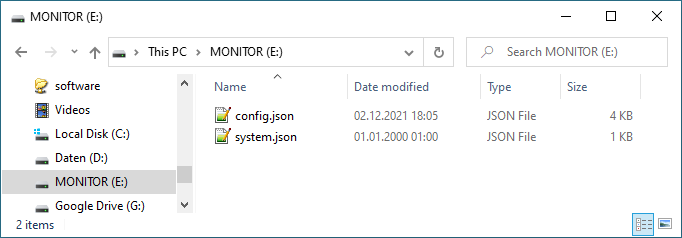
\includegraphics[width=13cm]{images/File_Explorer}
	\caption{Fleet-Monitor Root Directory}
	\label{fig:fleet-monitor-root-directory}
\end{figure}

Blablabla


\newpage

\subsection{Firmware Update} \label{Firmware Update}
\begin{wrapfigure}{r}{5.0cm}
\vspace{-0.6cm}
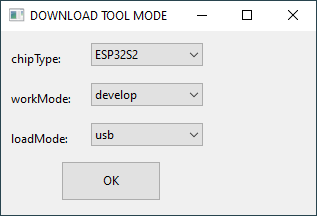
\includegraphics[width=5.0cm]{images/ESP32_Download_Mode}
\caption{ESP32 Download Tool}
\label{fig:esp32-download-tool}
\end{wrapfigure} 
bla bla bla bla bla bla bla bla bla bla bla bla bla bla bla bla bla bla bla bla bla bla bla bla bla bla bla bla bla bla bla bla bla bla bla bla bla bla bla bla bla bla bla bla bla bla bla bla bla bla bla bla bla bla bla bla bla bla bla bla bla bla bla bla bla bla bla bla bla bla bla bla bla bla bla bla bla bla bla bla bla bla bla bla bla bla bla bla bla bla bla bla bla bla bla bla bla bla bla bla bla bla bla bla bla bla bla bla bla bla bla bla bla bla bla bla bla bla bla bla bla bla bla 

Write about bootloader mode, update procedure
Path: \texttt{FleetMonitor$\backslash$.pio$\backslash$build$\backslash$esp32s2dev}
\cite{flash-download-tools}.


\begin{figure}[h!]
	\centering
	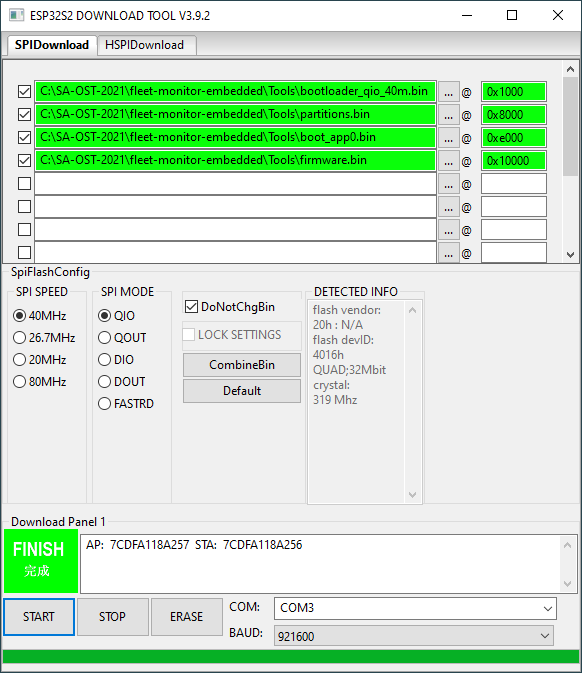
\includegraphics[width=11cm]{images/ESP32_Firmware_Settings}
	\caption{ESP32S2 Download Tool Settings}
	\label{fig:esp32s2-download-tool-settings}
\end{figure}
\newpage

\section{Specifications}
\todo{add more stuff}
\begin{center}
    \begin{tabular}{p{6.8cm} p{6.8cm}}
    \hline
    Input Voltage           & 9\,V - 28\,V                      \\ \hline
    Power Consumption       & 2.5\,W                            \\ \hline
    Water Resistance Rating & IP67                              \\ \hline  
    Microprocessor          & ESP32-S2                          \\ \hline
    LAN Interface           & 10Base-T / 100Base-TX             \\ \hline
    WLAN Interface          & 802,11b/g/n                       \\ \hline
    USB Interface           & USB 2.0 (Device)                  \\ \hline
    CAN Interface           & xxx\,kbit/s (SAE J1939)           \\ \hline
    
    \end{tabular}
\end{center}

\todo[inline]{Add CAN Frequency to Specifications}


\section{LED Status}
Luca

LED Status

\begin{center}
    \begin{tabular}{p{6.8cm} p{6.8cm}}
    \hline
    Input Voltage           & 9\,V - 28\,V  \\ \hline
    Power Consumption       & 2.5\,W        \\ \hline
    Microprocessor          & ESP32-S2      \\ \hline
    Water Resistance Rating & IP67          \\ \hline       
    \end{tabular}
\end{center}

LED CAN

\todo[inline]{Write about possible error scenarios and if the led is blinking red...}